
The translation of theoretical optimization frameworks into operational software systems demands careful attention to architectural design, component integration, and practical engineering considerations that extend well beyond algorithmic specification. This chapter provides a comprehensive treatment of the system architecture underlying reinforcement learning-optimized synthetic data generation for YOLO object detection training. The exposition progresses from high-level architectural overview through detailed examination of individual modules, culminating in practical guidance for implementation, deployment, and maintenance of production-grade optimization pipelines.

\section{Overall System Architecture}
\label{sec:system_architecture}

The complete optimization system comprises six principal modules that interact through well-defined interfaces to accomplish the overarching objective of discovering synthetic data generation parameters that maximize downstream detector performance on real-world validation imagery. The architectural philosophy embraces modularity, enabling independent development and testing of components while facilitating straightforward extension to novel generation backends, detection architectures, or optimization algorithms.

\subsection{End-to-End Pipeline Overview}

The optimization pipeline implements a closed-loop control system wherein the Optimization Controller proposes synthetic data generation parameter configurations, the Synthetic Data Generation Module renders training imagery according to these specifications, the YOLO Training Module trains detector models on the generated corpora, the Evaluation Module assesses trained models against held-out real-world validation data, and the Reward Computation Module transforms evaluation metrics into scalar feedback signals that inform subsequent parameter proposals. This iterative refinement process continues until convergence criteria are satisfied or computational budgets are exhausted.

The pipeline architecture reflects the expensive black-box optimization paradigm wherein each evaluation requires substantial computational investment spanning synthetic image rendering, neural network training, and inference on validation imagery. Consequently, the architecture prioritizes sample efficiency through intelligent parameter proposal via Tree-structured Parzen Estimation, early termination of unpromising trials through Hyperband pruning, and comprehensive state persistence enabling recovery from interruptions without loss of accumulated optimization progress.

Data flow through the system follows a unidirectional pattern during normal operation, with parameter configurations flowing from the Optimization Controller through generation and training to evaluation, while reward signals flow in the reverse direction to inform subsequent proposals. Bidirectional communication occurs during checkpointing operations when module states are persisted to durable storage, and during warm-start initialization when prior optimization results are loaded to accelerate convergence on related problems.

\subsection{Component Interaction Architecture}

The interaction patterns among system components reflect careful consideration of computational dependencies, failure isolation, and resource utilization efficiency. The Optimization Controller serves as the central orchestrator, maintaining the optimization study state and coordinating the execution of individual trials. Upon initialization, the Controller queries persistent storage to determine whether a prior study exists for resumption or whether a fresh optimization campaign should commence.

For each trial, the Controller invokes the parameter proposal mechanism to generate a candidate configuration, instantiates the Synthetic Data Generation Module with the proposed parameters, awaits completion of the rendering process, configures the YOLO Training Module with appropriate hyperparameters and data paths, monitors training progress through callback interfaces that enable early termination decisions, invokes the Evaluation Module upon training completion to assess model performance, computes reward signals through the Reward Computation Module, and records the complete trial history to persistent storage before proposing the next configuration.

The modular architecture enables parallel execution of independent operations through asynchronous trial management. Multiple synthetic data generation processes may execute concurrently on available computational resources, and the Controller maintains a pool of pending evaluations that are dispatched as GPU resources become available. This parallelization strategy substantially reduces wall-clock time to convergence while maintaining the sequential dependencies inherent in the optimization algorithm.

\begin{figure}[htbp]
\centering
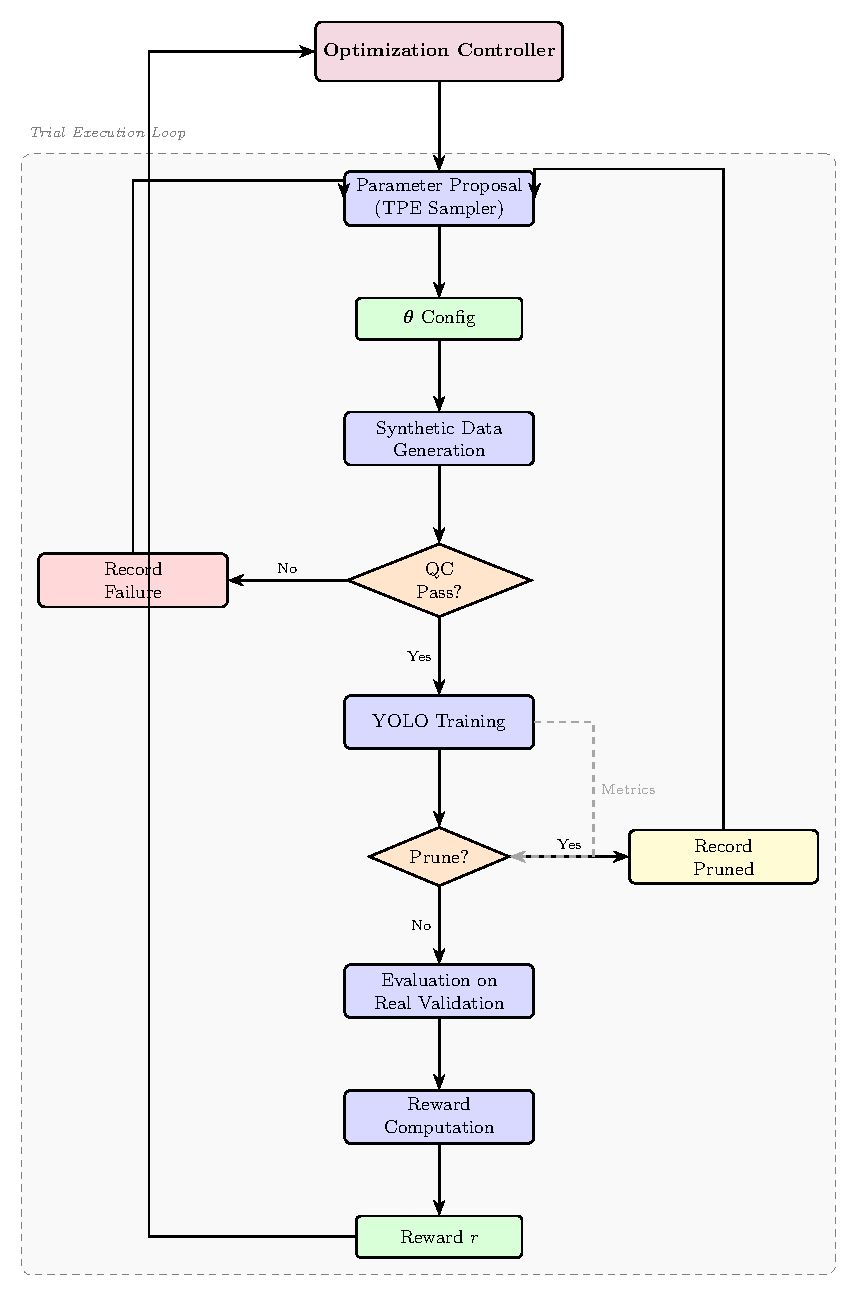
\includegraphics[width=0.75\textwidth]{figures/ch09_fig1_component_interaction.pdf}
\caption{Trial execution flowchart depicting the sequence of operations within each optimization trial. The Optimization Controller orchestrates parameter proposal through the TPE sampler, synthetic data generation, YOLO training with pruning evaluation, and reward computation. Decision diamonds indicate quality control and pruning checkpoints where trials may be terminated early. Dashed feedback paths show how intermediate training metrics inform pruning decisions and how reward signals guide subsequent parameter proposals.}
\label{fig:component_interaction}
\end{figure}

\subsection{System Architecture Diagram}

The following diagram illustrates the complete system architecture, depicting the six principal modules, their interconnections, and the flow of data and control signals throughout the optimization loop.

\begin{figure}[htbp]
\centering
\begin{tikzpicture}[
    node distance=1.8cm and 2.5cm,
    module/.style={rectangle, draw=black, thick, fill=blue!10, minimum width=4cm, minimum height=1.2cm, align=center, rounded corners=3pt},
    storage/.style={cylinder, draw=black, thick, fill=orange!20, shape border rotate=90, aspect=0.25, minimum width=2.5cm, minimum height=1cm, align=center},
    process/.style={rectangle, draw=black, thick, fill=green!10, minimum width=3.5cm, minimum height=1cm, align=center, rounded corners=3pt},
    arrow/.style={->, thick, >=stealth},
    dataarrow/.style={->, thick, >=stealth, color=blue!70},
    ctrlarrow/.style={->, thick, >=stealth, color=red!70, dashed}
]

% Main modules
\node[module] (optctrl) {\textbf{Optimization Controller}\\Optuna Study Manager};
\node[module, below=of optctrl] (synth) {\textbf{Synthetic Data Generation}\\Blender / Isaac Sim};
\node[module, below=of synth] (yolo) {\textbf{YOLO Training Module}\\Ultralytics Integration};
\node[module, right=3.5cm of yolo] (eval) {\textbf{Evaluation Module}\\Real Validation Assessment};
\node[module, right=3.5cm of synth] (reward) {\textbf{Reward Computation}\\Multi-Objective Aggregation};

% Storage components
\node[storage, left=2.5cm of optctrl] (studydb) {Study\\Database};
\node[storage, left=2.5cm of synth] (imgstore) {Image\\Storage};
\node[storage, left=2.5cm of yolo] (ckptstore) {Checkpoint\\Storage};
\node[storage, right=3.5cm of optctrl] (logstore) {Metrics\\Logs};

% Data flow arrows
\draw[dataarrow] (optctrl) -- node[left, font=\small] {Parameters} (synth);
\draw[dataarrow] (synth) -- node[left, font=\small] {Training Data} (yolo);
\draw[dataarrow] (yolo) -- node[below, font=\small] {Trained Model} (eval);
\draw[dataarrow] (eval) -- node[right, font=\small] {Metrics} (reward);
\draw[dataarrow] (reward) -- node[above, font=\small] {Reward Signal} (optctrl);

% Storage connections
\draw[arrow] (optctrl) -- (studydb);
\draw[arrow] (synth) -- (imgstore);
\draw[arrow] (yolo) -- (ckptstore);
\draw[arrow] (reward) -- (logstore);

% Control flow
\draw[ctrlarrow] (optctrl.south west) to[out=-150, in=150] node[left, font=\small, color=red!70] {Trial Control} (yolo.north west);

% Legend
\node[below=3.5cm of yolo, xshift=-2cm] (legend) {};
\draw[dataarrow] (legend) -- ++(1.5,0) node[right, font=\small] {Data Flow};
\draw[ctrlarrow] ([yshift=-0.5cm]legend) -- ++(1.5,0) node[right, font=\small] {Control Signal};

\end{tikzpicture}
\caption{System architecture diagram depicting the six principal modules and their interconnections. Blue solid arrows indicate data flow paths carrying parameters, images, models, and metrics. Red dashed arrows indicate control signals for trial management and early termination. Cylindrical nodes represent persistent storage components for study state, generated imagery, model checkpoints, and optimization logs.}
\label{fig:system_architecture}
\end{figure}

\subsection{Data Flow Through the System}

The data transformation pipeline begins with the Optimization Controller generating a parameter vector $\boldsymbol{\theta} \in \Theta$ specifying the complete configuration for synthetic data generation. This vector encompasses continuous parameters such as lighting intensity ranges and object scale bounds, discrete parameters such as the number of distractor objects per scene, and categorical parameters such as background environment selection. The parameter vector is serialized and transmitted to the Synthetic Data Generation Module along with metadata specifying the desired corpus size and output format.

The Synthetic Data Generation Module interprets the parameter vector to configure its internal randomization engine, procedurally generates the specified number of training images with corresponding annotations, performs quality assurance validation on the generated corpus, and writes the imagery and annotation files to designated storage locations. The module returns a manifest file specifying the paths to generated assets along with summary statistics describing the realized parameter distributions, enabling verification that the stochastic generation process produced outputs consistent with the specified configuration.

The YOLO Training Module consumes the generated corpus manifest to configure data loading pipelines, initializes model weights either from scratch or from a provided pretrained checkpoint, executes the training loop with periodic validation against a held-out synthetic validation subset, and persists model checkpoints at configurable intervals. Throughout training, the module exposes progress metrics through callback interfaces that enable the Optimization Controller to make pruning decisions based on intermediate performance indicators.

Upon training completion, the Evaluation Module loads the final model checkpoint and executes inference on the real-world validation set. The module computes comprehensive detection metrics including mean Average Precision at multiple Intersection over Union thresholds, per-class precision and recall statistics, and inference latency measurements. These metrics are aggregated into a structured evaluation report that is transmitted to the Reward Computation Module.

The Reward Computation Module transforms the multi-dimensional evaluation report into a scalar reward signal suitable for optimization algorithm consumption. This transformation involves normalization relative to historical performance distributions, application of weighting coefficients reflecting relative objective importance, detection and penalization of degenerate solutions, and optional temporal smoothing to reduce reward variance across stochastic training runs. The computed reward is returned to the Optimization Controller, completing the feedback loop and enabling informed proposal of subsequent parameter configurations.

\section{Synthetic Data Generation Module}
\label{sec:synth_data_module}

The Synthetic Data Generation Module bears responsibility for translating abstract parameter specifications into concrete training imagery that, despite its synthetic origin, induces detector representations capable of generalizing to real-world deployment scenarios. The module architecture supports multiple rendering backends through a unified abstraction layer, enabling practitioners to select generation engines appropriate to their specific domain requirements and computational resources.

\subsection{Blender and Isaac Sim Integration}

The module provides native integration with two primary rendering backends that collectively address the majority of synthetic data generation requirements encountered in practice. NVIDIA Isaac Sim, built upon the Omniverse platform, offers production-grade physics simulation, photorealistic path-traced rendering through the RTX renderer, and extensive libraries of simulation-ready assets with embedded semantic annotations. Isaac Sim integration is accomplished through the Omniverse Replicator API, which exposes programmatic control over scene composition, randomization parameters, and annotation generation through Python scripting interfaces.

Blender integration leverages the open-source three-dimensional creation suite's comprehensive Python API to achieve comparable functionality with reduced licensing complexity and hardware requirements. The Cycles rendering engine provides physically-based path tracing capable of photorealistic output, while the Eevee engine offers substantially faster rasterization-based rendering suitable for rapid prototyping and exploration phases of optimization campaigns. Blender's extensive material system supports physically-based rendering workflows with metallic, roughness, and normal mapping that accurately simulate real-world surface appearance under varied illumination conditions.

The backend abstraction layer defines a common interface through which the Optimization Controller interacts with either rendering engine without modification. This interface specifies methods for scene initialization, parameter application, frame rendering, and annotation export, enabling transparent backend substitution based on deployment requirements. The abstraction layer additionally provides automatic format conversion utilities that transform backend-specific annotation formats into the YOLO-compatible format required by downstream training pipelines.

\subsection{Parameter Space Definition}

The parameter space governing synthetic data generation encompasses multiple categories of configurable attributes, each contributing distinct aspects of visual variation to the generated corpus. The module maintains a hierarchical parameter specification that organizes individual parameters into semantically coherent groups while exposing the complete flattened vector to the optimization algorithm.

Object appearance parameters control the visual properties of target detection objects, encompassing texture selection from curated material libraries, color variation through hue-saturation-value perturbation, surface finish properties including metalness and roughness coefficients, and subsurface scattering parameters for translucent materials. These parameters collectively determine the feature distributions that trained detectors must recognize across the range of visual appearances exhibited by real-world objects.

Geometric variation parameters govern the spatial configuration of scene elements, including object position distributions within the scene volume, rotation distributions specifying allowable orientations, scale distributions defining size variation ranges, and aspect ratio perturbations that introduce controlled geometric distortion. Physics-based placement algorithms optionally simulate gravitational settling to achieve naturalistic object arrangements that avoid interpenetration artifacts.

Illumination parameters control the synthetic lighting environment, encompassing the number, positions, and intensities of point and area light sources, ambient illumination levels from environment maps, shadow characteristics determined by light source geometry, and color temperature variation spanning the range from warm tungsten to cool daylight illumination. High dynamic range environment maps provide image-based lighting that captures complex real-world illumination patterns including indirect reflections and color bleeding effects.

Camera parameters specify the virtual sensor configuration, including focal length determining field of view and perspective distortion characteristics, sensor dimensions affecting image resolution and aspect ratio, lens distortion coefficients modeling barrel and pincushion aberrations, and depth of field parameters when bokeh simulation is desired. Motion blur simulation parameters enable generation of imagery exhibiting the temporal integration artifacts characteristic of moving cameras or subjects.

Environmental parameters introduce scene-level variation through weather simulation including rain, fog, and snow effects, time-of-day variation affecting solar illumination angle and color, and atmospheric scattering models that introduce depth-dependent color shifts. Background variation parameters control the selection and configuration of scene backdrops ranging from solid colors through photographic backgrounds to fully three-dimensional environment geometry.

\begin{table}[htbp]
\centering
\caption{Synthetic Data Generation Parameter Categories and Typical Ranges}
\label{tab:parameter_space}
\begin{tabular}{p{3cm}p{4cm}p{3cm}p{4cm}}
\toprule
\textbf{Category} & \textbf{Parameter} & \textbf{Type} & \textbf{Typical Range} \\
\midrule
Object Appearance & Texture Library Index & Categorical & Domain-specific \\
 & Hue Variation & Continuous & $[-30, +30]$ degrees \\
 & Saturation Scale & Continuous & $[0.7, 1.3]$ \\
 & Metalness & Continuous & $[0.0, 1.0]$ \\
 & Roughness & Continuous & $[0.1, 0.9]$ \\
\addlinespace
Geometric & Position X/Y/Z & Continuous & Scene-dependent \\
 & Rotation Range & Continuous & $[0, 360]$ degrees \\
 & Scale Factor & Continuous & $[0.5, 2.0]$ \\
 & Object Count & Discrete & $[1, 20]$ \\
\addlinespace
Illumination & Light Count & Discrete & $[1, 8]$ \\
 & Intensity Range & Continuous & $[0.2, 5.0]$ \\
 & Color Temperature & Continuous & $[2700, 6500]$ Kelvin \\
 & Ambient Ratio & Continuous & $[0.1, 0.5]$ \\
\addlinespace
Camera & Focal Length & Continuous & $[24, 85]$ mm \\
 & Sensor Height & Continuous & Match deployment \\
 & Distortion k1 & Continuous & $[-0.3, 0.3]$ \\
\addlinespace
Environment & Fog Density & Continuous & $[0.0, 0.5]$ \\
 & Rain Intensity & Continuous & $[0.0, 1.0]$ \\
 & Time of Day & Continuous & $[0, 24]$ hours \\
\bottomrule
\end{tabular}
\end{table}

\subsection{Randomization Controller}

The Randomization Controller implements the stochastic sampling mechanisms that translate parameter specifications into concrete per-frame configurations. For each rendered frame, the Controller samples values from the distributions defined by the current parameter vector, applies these values to configure the scene state, and records the realized values in the frame metadata for subsequent analysis and debugging purposes.

The Controller supports multiple distribution families for continuous parameters, including uniform distributions for parameters with equally likely values throughout the specified range, truncated Gaussian distributions for parameters with preferred central values and diminishing probability toward range boundaries, and log-uniform distributions for parameters spanning multiple orders of magnitude such as lighting intensities. Discrete parameters employ categorical distributions with configurable probability masses for each allowable value.

Correlation structures among parameters are optionally specified through the parameter configuration, enabling the Controller to generate coherent multi-parameter variations that reflect real-world covariance patterns. For instance, outdoor illumination intensity and color temperature exhibit strong correlation in natural environments, with high intensities typically accompanying neutral color temperatures and low intensities accompanying warmer temperatures. The Controller implements Gaussian copula sampling to generate parameter vectors respecting specified correlation matrices while maintaining marginal distributions conforming to parameter-specific requirements.

The Controller additionally implements stratified sampling strategies that ensure systematic coverage of the parameter space across the generated corpus. Rather than independent sampling for each frame, stratified sampling partitions the parameter space into strata and generates equal numbers of samples from each stratum, reducing clustering artifacts and improving training data diversity for fixed corpus sizes. Latin hypercube sampling provides an efficient implementation of this strategy for high-dimensional parameter spaces.

\subsection{Annotation Generation in YOLO Format}

The annotation generation subsystem produces ground truth labels in the format expected by YOLO training pipelines, specifically normalized bounding box coordinates accompanied by integer class identifiers. For each rendered frame, the subsystem projects three-dimensional object bounding volumes into image coordinates, computes axis-aligned two-dimensional bounding rectangles enclosing the projected volumes, filters annotations for objects with insufficient visibility due to occlusion or frame boundary truncation, normalizes coordinates relative to image dimensions, and writes annotation files in the standard YOLO text format with one annotation per line.

Visibility computation accounts for occlusion by other scene objects through depth buffer analysis, determining the fraction of each object's projected area that remains unoccluded in the final rendered image. Objects with visibility below a configurable threshold are excluded from the annotation set to avoid training the detector on severely occluded instances that would be difficult to recognize even for human annotators. The visibility threshold represents a tunable parameter that balances training data completeness against annotation reliability.

The subsystem additionally generates segmentation masks and keypoint annotations when supported by the target detection architecture, enabling training of instance segmentation and pose estimation models alongside standard bounding box detectors. These extended annotations leverage the complete scene geometry information available in the synthetic environment to produce pixel-perfect ground truth that would require substantial manual effort to obtain for real-world imagery.

\subsection{Quality Assurance Checks}

The Quality Assurance subsystem validates generated imagery and annotations against configurable acceptance criteria, flagging or rejecting frames that fail to meet quality standards. Validation checks encompass both low-level image quality metrics and high-level semantic consistency requirements that collectively ensure the generated corpus provides effective training signal for downstream detector models.

Image quality validation verifies that rendered frames exhibit appropriate exposure levels without excessive clipping in highlight or shadow regions, sufficient contrast to enable feature extraction, absence of rendering artifacts such as fireflies in path-traced output, and spatial resolution adequate for detecting the smallest target objects. Frames failing quality thresholds trigger re-rendering with adjusted random seeds, ensuring that quality failures do not reduce the effective corpus size.

Annotation quality validation confirms that generated labels satisfy integrity constraints including non-empty annotation sets for frames containing target objects, bounding box coordinates within valid normalized ranges, class identifiers corresponding to defined object categories, and absence of degenerate boxes with zero area. The validation subsystem additionally computes corpus-level statistics including class balance ratios and object size distributions, flagging configurations that produce severely imbalanced or degenerate datasets.

\begin{figure}[htbp]
\centering
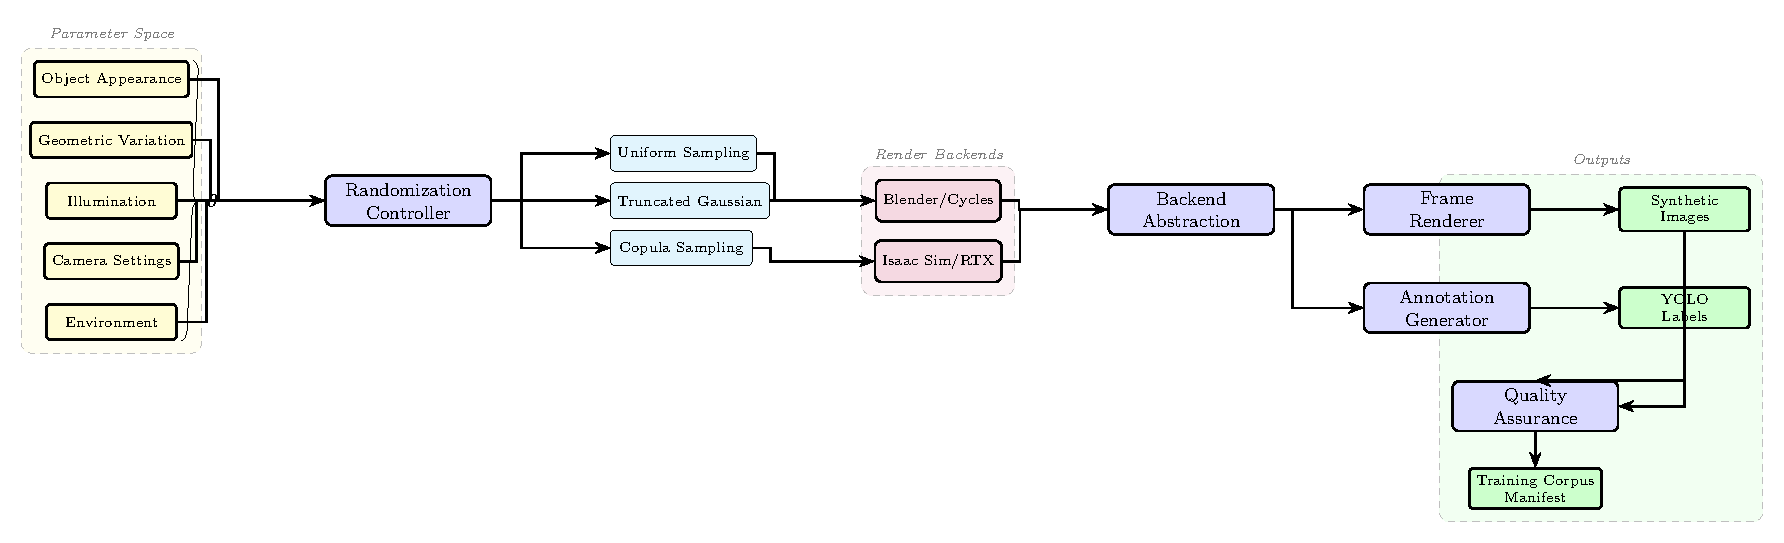
\includegraphics[width=\textwidth]{figures/ch09_fig2_synth_data_pipeline.pdf}
\caption{Synthetic data generation pipeline architecture. Parameter specifications flow from the parameter space through the Randomization Controller, which selects appropriate sampling strategies (uniform, truncated Gaussian, or copula-based) based on parameter characteristics. The rendering backend abstraction layer enables transparent switching between Blender and Isaac Sim engines. The pipeline produces synthetic images and YOLO-format annotations that undergo quality assurance validation before being assembled into the training corpus manifest.}
\label{fig:synth_data_pipeline}
\end{figure}

\section{YOLO Training Module}
\label{sec:yolo_training_module}

The YOLO Training Module encapsulates the complete neural network training workflow, providing a consistent interface through which the optimization system interacts with the underlying detection architecture regardless of the specific YOLO variant employed. The module architecture separates configuration management, training execution, and progress monitoring into distinct subsystems that collectively enable reliable automated training across diverse hardware configurations and experimental conditions.

\subsection{Ultralytics Integration}

The module achieves YOLO training capabilities through integration with the Ultralytics library, which provides production-grade implementations of YOLOv5, YOLOv8, and subsequent architecture revisions with consistent training APIs. Ultralytics integration is accomplished through programmatic invocation of the library's training entry points with configuration parameters derived from the optimization system's trial specifications.

The integration layer translates between the optimization system's internal parameter representation and the Ultralytics configuration format, mapping synthetic data generation parameters to data loader configurations, optimization hyperparameters to training settings, and architecture specifications to model constructors. This translation layer insulates the optimization system from implementation details of specific Ultralytics versions, enabling library upgrades without modification to the optimization codebase.

The integration additionally exposes Ultralytics callback interfaces to the optimization system, enabling registration of custom callbacks for progress monitoring, intermediate validation, and early termination. These callbacks receive training state information including current epoch, batch loss values, and validation metrics, transmitting this information to the Optimization Controller for pruning decisions and progress logging.

\subsection{Configuration Management}

The Configuration Management subsystem maintains hierarchical configuration structures that specify all parameters governing YOLO training execution. Configuration parameters are organized into categories encompassing model architecture selection, data augmentation strategies, optimization algorithm settings, learning rate scheduling, regularization techniques, and resource allocation directives.

Model architecture configuration specifies the YOLO variant and scale to employ, selecting among available backbone networks and head configurations. The configuration supports specification of pretrained weight paths for transfer learning scenarios, random weight initialization for training from scratch, and partial weight loading for architecture modification experiments. Input resolution configuration determines the spatial dimensions of images processed by the network, with implications for detection performance on small objects and computational resource requirements.

Data augmentation configuration controls the online augmentation pipeline applied to training images, specifying augmentation operations and their associated probability and magnitude parameters. Standard augmentations include geometric transformations such as scaling, rotation, and horizontal flipping, color space transformations such as hue, saturation, and brightness adjustment, and composite augmentations such as mosaic combining multiple training images into single inputs. Augmentation parameters may be fixed throughout optimization or included in the optimization parameter space for joint tuning with generation parameters.

Optimization configuration specifies the gradient descent algorithm, learning rate values and scheduling policies, batch size and gradient accumulation settings, and weight decay regularization strength. The subsystem supports SGD with momentum, Adam, and AdamW optimizers with configurable hyperparameters, along with learning rate schedulers including step decay, cosine annealing, and one-cycle policies.

\subsection{Checkpoint Handling}

The Checkpoint Handling subsystem manages model state persistence throughout training execution, enabling recovery from interruptions and provision of trained models to downstream evaluation. Checkpoints are persisted at configurable epoch intervals, with special handling for best-performing checkpoints determined by validation metrics and final-epoch checkpoints representing training completion.

The subsystem implements intelligent checkpoint retention policies that balance storage requirements against recovery capabilities. The rolling retention policy maintains only the most recent checkpoint along with the best-performing checkpoint, minimizing storage consumption while preserving the ability to resume from interruption and access peak-performance weights. The complete retention policy maintains all checkpoints throughout training, enabling detailed analysis of training dynamics at the cost of substantially increased storage requirements.

Checkpoint files include complete model state dictionaries, optimizer state enabling exact training resumption, epoch counters and learning rate scheduler states, and metadata describing the training configuration and data corpus. The standardized checkpoint format ensures compatibility with Ultralytics inference utilities and third-party analysis tools.

\subsection{Metrics Logging}

The Metrics Logging subsystem instruments training execution to capture comprehensive performance measurements enabling optimization algorithm feedback and experimental analysis. Logged metrics encompass training loss components, validation metrics, learning rate values, and timing measurements for each training epoch.

Training loss logging captures the individual loss components contributing to the total optimization objective, including objectness loss quantifying confidence calibration, classification loss measuring class prediction accuracy, and bounding box regression loss assessing localization precision. Component-level logging enables diagnosis of training dynamics and identification of loss terms dominating the optimization landscape.

Validation metrics logging records detector performance on held-out validation subsets at configurable intervals throughout training. Standard metrics include mean Average Precision at IoU threshold 0.50, mean Average Precision averaged across IoU thresholds from 0.50 to 0.95, and per-class Average Precision values enabling analysis of class-specific performance variation. These intermediate validation metrics provide the signals consumed by pruning algorithms for early termination decisions.

The logging subsystem integrates with standard experiment tracking platforms including TensorBoard, Weights and Biases, and MLflow, enabling visualization of training curves and comparison across optimization trials. Integration is accomplished through callback registration during training initialization, with the specific tracking platform selected through configuration parameters.

\subsection{GPU Resource Management}

The GPU Resource Management subsystem coordinates allocation of graphics processing resources across concurrent training workloads, ensuring efficient utilization while preventing resource contention that would degrade training throughput. The subsystem maintains awareness of available GPU devices, their memory capacities, and current utilization levels, informing scheduling decisions that maximize aggregate training throughput.

Device allocation policies specify how training workloads are assigned to available GPUs, ranging from exclusive allocation wherein each training process receives dedicated GPU resources through shared allocation wherein multiple lightweight processes time-slice a single device. The appropriate policy depends on model scale, batch size requirements, and the number of concurrent trials supported by the optimization configuration.

Memory management utilities monitor GPU memory utilization throughout training, implementing proactive batch size reduction when memory pressure exceeds configurable thresholds and gradient checkpointing activation when model scale approaches device memory limits. These adaptive mechanisms enable robust training execution across varied hardware configurations without manual tuning of memory-related hyperparameters.

Multi-GPU training support enables distribution of single training workloads across multiple devices through data parallelism, with automatic gradient synchronization and batch splitting managed by the underlying Ultralytics infrastructure. The Resource Management subsystem exposes configuration options for multi-GPU allocation and handles the additional complexity of coordinating distributed training with the checkpoint and metrics logging subsystems.

\section{Evaluation Module}
\label{sec:evaluation_module}

The Evaluation Module assesses trained detector performance against held-out real-world validation imagery, producing the performance metrics that ultimately determine optimization success. The module architecture addresses the statistical challenges inherent in evaluation with limited validation data, implementing robust estimation procedures that provide reliable performance signals despite validation set sizes that may be as small as fifty images.

\subsection{Real Validation Set Management}

The Validation Set Management subsystem maintains the real-world imagery corpus against which trained detectors are evaluated, ensuring consistent evaluation conditions across optimization trials while supporting validation set updates as additional real-world data becomes available. The validation set is isolated from synthetic training data through directory structure conventions and explicit path configuration, eliminating the possibility of data leakage that would inflate performance estimates.

The subsystem implements stratified subset selection utilities that construct evaluation batches balanced across object categories, ensuring that per-class performance metrics reflect evaluation on representative samples of each category. Stratification is accomplished through iterative selection that prioritizes images containing underrepresented categories until target class frequencies are achieved or the complete validation set is exhausted.

Validation set versioning enables tracking of evaluation corpus evolution across optimization campaigns, with checksum-based integrity verification ensuring that performance comparisons across trials employ identical evaluation data. The versioning system maintains association between trial results and validation set versions, enabling principled interpretation of historical results when validation sets are augmented with newly acquired real-world imagery.

Preprocessing pipelines applied to validation imagery are explicitly configured and version-controlled alongside the imagery itself, ensuring that evaluation conditions remain reproducible. Standard preprocessing operations include resolution normalization to match training input dimensions, color space conversion if required by the detection architecture, and optional test-time augmentation that evaluates each image under multiple transformations to improve prediction robustness.

\subsection{Bootstrap Confidence Computation}

The Bootstrap Confidence subsystem quantifies the statistical uncertainty associated with performance estimates derived from limited validation data, enabling principled comparison of detector performance across optimization trials and meaningful assessment of whether observed performance differences exceed expected sampling variation.

Bootstrap resampling constructs multiple pseudo-validation sets by sampling with replacement from the original validation corpus, computing detection metrics on each resampled set to generate an empirical distribution of performance estimates. Standard bootstrap procedures draw one thousand or more resamples, with the resampled metric distribution characterizing the statistical uncertainty attributable to validation set composition.

Confidence interval construction employs the percentile method, reporting the 2.5th and 97.5th percentiles of the bootstrap distribution as the bounds of a 95\% confidence interval. The bias-corrected and accelerated (BCa) bootstrap variant provides improved coverage properties when the sampling distribution exhibits skewness, as commonly occurs for bounded metrics such as precision and recall that approach their theoretical limits.

Statistical comparison utilities employ bootstrap hypothesis testing to determine whether performance differences between detector variants achieve statistical significance. The null hypothesis of equal population performance is evaluated by constructing a bootstrap distribution of performance differences and determining whether zero falls outside the resulting confidence interval. This procedure provides principled guidance for selecting among detector variants when observed performance differences are modest relative to sampling uncertainty.

\subsection{Class-Balanced mAP Calculation}

The Class-Balanced mAP subsystem computes mean Average Precision metrics that weight category contributions according to principled schemes reflecting application requirements, addressing the limitation of standard mAP computation wherein rare categories contribute minimally to aggregate scores despite their potential importance for deployment success.

Standard mAP computation averages per-class Average Precision values with uniform weights, implicitly prioritizing categories proportionally to their representation in the validation set. For imbalanced validation corpora where category frequencies diverge substantially from uniform distribution, this weighting scheme permits high aggregate scores while tolerating poor performance on underrepresented categories.

Class-balanced weighting assigns equal importance to each category regardless of validation set representation, computing the arithmetic mean of per-class Average Precision values. This scheme ensures that optimization pressure applies equally across categories, preventing the optimizer from discovering configurations that sacrifice rare-category performance to maximize aggregate metrics dominated by common categories.

Frequency-inverse weighting assigns category weights inversely proportional to validation set frequencies, amplifying the contribution of rare categories beyond equal weighting. This aggressive rebalancing scheme is appropriate when rare categories correspond to high-consequence detection targets whose reliable identification justifies disproportionate optimization effort.

The subsystem reports multiple mAP variants simultaneously, enabling practitioners to select the weighting scheme most appropriate for their application while monitoring alternative metrics for diagnostic purposes. Disagreement between uniformly-weighted and class-balanced metrics signals class-conditional performance variation that warrants investigation regardless of the primary optimization objective.

\subsection{Result Caching and History}

The Result Caching subsystem maintains persistent records of evaluation results across optimization campaigns, enabling historical analysis, reproducibility verification, and warm-starting of subsequent optimization runs from prior accumulated knowledge. The caching architecture separates ephemeral computation state from durable result records, ensuring that evaluation history survives system restarts and infrastructure changes.

The caching database records complete trial specifications including synthetic data generation parameters, training hyperparameters, random seeds, and software version identifiers alongside evaluation results encompassing all computed metrics and their bootstrap confidence intervals. This comprehensive recording enables post-hoc analysis of parameter-performance relationships, identification of promising parameter regions for focused exploration, and diagnosis of optimization pathologies.

Cache invalidation policies specify conditions under which cached results are discarded and recomputation triggered, addressing scenarios where cached results no longer reflect current system behavior. Invalidation triggers include validation set modifications, evaluation procedure changes, and detection of hardware-dependent result variation. Conservative invalidation policies that preserve cache entries across minor system changes maximize the value of accumulated evaluation history while accepting the risk of stale results under certain edge conditions.

History visualization utilities generate summary plots depicting optimization progress over trial sequences, parameter importance rankings derived from cached results, and performance-parameter scatter plots illuminating the optimization landscape structure. These visualizations support interactive exploration of optimization campaigns, informing parameter space refinement and identification of convergence to local optima.

\section{Optimization Controller}
\label{sec:optimization_controller}

The Optimization Controller implements the Bayesian optimization algorithm that proposes parameter configurations, manages trial execution, and maintains optimization state across potentially long-running campaigns. The Controller architecture employs the Optuna framework as its optimization backend, leveraging Optuna's sophisticated sampling algorithms, pruning mechanisms, and distributed execution capabilities while providing application-specific extensions for synthetic data optimization.

\subsection{Optuna Study Configuration}

Study configuration specifies the high-level structure of the optimization problem including the optimization direction, parameter space definition, and study persistence settings. The optimization direction indicates whether the objective should be maximized or minimized, with mAP optimization specifying maximization while loss-based objectives would specify minimization.

The parameter space definition enumerates all tunable parameters along with their types and domains, constructed from the union of synthetic data generation parameters, training hyperparameters, and optionally augmentation parameters. Continuous parameters specify lower and upper bounds along with optional distribution hints that inform the sampling algorithm. Discrete parameters enumerate allowable values with optional ordering information. Categorical parameters specify the set of allowable string or integer identifiers without implied ordering.

Study persistence configuration specifies the storage backend maintaining optimization state across Controller invocations. SQLite storage provides simple single-file persistence suitable for single-machine optimization campaigns. PostgreSQL storage enables distributed optimization with multiple workers proposing and evaluating trials concurrently while maintaining consistent study state. Redis storage provides in-memory persistence with optional durability, offering reduced latency for high-frequency trial operations at the cost of increased infrastructure complexity.

\begin{table}[htbp]
\centering
\caption{Optuna Study Configuration Parameters}
\label{tab:optuna_config}
\begin{tabular}{p{3.5cm}p{3cm}p{6.5cm}}
\toprule
\textbf{Parameter} & \textbf{Default Value} & \textbf{Description} \\
\midrule
study\_name & Required & Unique identifier for the optimization study \\
direction & maximize & Optimization direction for the primary objective \\
storage & sqlite:///study.db & Database URL for study persistence \\
load\_if\_exists & True & Resume existing study if present \\
n\_startup\_trials & 10 & Random trials before TPE sampling begins \\
n\_ei\_candidates & 24 & Candidates evaluated for expected improvement \\
multivariate & True & Model parameter correlations in TPE \\
\bottomrule
\end{tabular}
\end{table}

\subsection{TPE Sampler Setup}

The Tree-structured Parzen Estimator sampler implements the parameter proposal mechanism that balances exploration of unvisited parameter regions against exploitation of promising regions identified through prior evaluations. TPE constructs separate density models over parameter configurations yielding above-threshold and below-threshold objective values, proposing configurations that maximize the ratio of above-threshold to below-threshold density.

Startup trial configuration specifies the number of initial trials sampled uniformly at random before TPE modeling commences. Sufficient startup trials ensure that the TPE model receives diverse observations spanning the parameter space, preventing premature convergence to local optima based on unrepresentative initial samples. The recommended startup count scales with parameter dimensionality, with ten trials providing adequate coverage for optimization problems with fewer than fifteen parameters.

Candidate evaluation count determines the number of parameter configurations evaluated during acquisition function optimization, with the highest-scoring candidate selected for the next trial. Larger candidate counts provide more thorough acquisition function optimization at the cost of increased computational overhead, with twenty-four candidates representing a reasonable balance for typical optimization problems.

Multivariate modeling enables the TPE sampler to capture correlations among parameters, constructing joint density models rather than independent per-parameter models. Multivariate modeling improves sample efficiency when parameters interact strongly, as commonly occurs in synthetic data generation where lighting and material parameters jointly determine rendered appearance. The computational overhead of multivariate modeling scales polynomially with parameter count, potentially necessitating independent modeling for high-dimensional problems.

\subsection{Hyperband Pruner Configuration}

The Hyperband pruner implements early termination of unpromising trials based on intermediate performance measurements, substantially reducing computational expenditure by abandoning trials whose trajectory indicates low probability of achieving competitive final performance. Hyperband extends successive halving to automatically determine appropriate resource allocation without requiring manual specification of the exploration-exploitation tradeoff.

Minimum resource configuration specifies the earliest training stage at which pruning decisions are considered, preventing premature termination based on unreliable early-training metrics. For YOLO training, minimum resource is typically specified in epochs, with values between five and fifteen epochs ensuring that pruning decisions reflect model behavior beyond random initialization.

Maximum resource configuration specifies the full training budget assigned to unpruned trials that survive all intermediate evaluations. The ratio of maximum to minimum resource determines the reduction factor applied at each pruning stage, with trials surviving each stage receiving multiplicatively increased resources until reaching the maximum allocation.

Reduction factor determines the fraction of trials promoted at each successive halving stage, with larger reduction factors providing more aggressive pruning at the cost of increased risk of discarding trials that would ultimately achieve strong performance. The default reduction factor of three retains one-third of trials at each stage, providing a reasonable balance between computational savings and optimization reliability.

\begin{table}[htbp]
\centering
\caption{Hyperband Pruner Configuration Parameters}
\label{tab:hyperband_config}
\begin{tabular}{p{3.5cm}p{3cm}p{6.5cm}}
\toprule
\textbf{Parameter} & \textbf{Default Value} & \textbf{Description} \\
\midrule
min\_resource & 1 & Minimum budget before pruning eligibility \\
max\_resource & auto & Maximum budget for complete trials \\
reduction\_factor & 3 & Fraction of trials surviving each stage \\
bootstrap\_count & 0 & Startup trials before pruning begins \\
\bottomrule
\end{tabular}
\end{table}

\subsection{Trial Management}

The Trial Management subsystem coordinates the lifecycle of individual optimization trials from parameter proposal through evaluation completion, handling both successful completions and various failure modes that may interrupt trial execution. Trial state transitions follow a well-defined state machine with states for running, complete, pruned, and failed trials.

Trial initialization allocates a unique trial identifier, samples parameter values from the configured sampler, records the proposed configuration to persistent storage, and transitions the trial to running state. The parameter sampling process queries the sampler with the current trial handle, enabling the sampler to access the complete optimization history when generating proposals.

Trial execution invokes the synthetic data generation, training, and evaluation pipeline with the proposed parameters, reporting intermediate metrics to the pruner at configurable intervals. Intermediate reporting enables pruning decisions during training execution, avoiding the computational waste of completing training runs whose intermediate performance indicates poor final outcomes.

Trial completion records final evaluation metrics to the study database and transitions the trial to completed state. The completion handler additionally updates sampler state with the new observation, enabling subsequent proposals to benefit from the accumulated evaluation history. Failed trials resulting from infrastructure errors or invalid parameter combinations transition to failed state with recorded failure reasons, excluding their results from sampler modeling while preserving diagnostic information.

\subsection{Database Persistence}

The Database Persistence subsystem maintains durable records of optimization state enabling recovery from system failures, analysis of optimization history, and coordination among distributed optimization workers. The persistence architecture employs relational database storage with a schema capturing studies, trials, parameter values, and intermediate results.

The study table maintains high-level study metadata including study names, creation timestamps, optimization directions, and study-level configuration. The trial table records individual trials with foreign key references to parent studies, capturing trial states, objective values, and completion timestamps. The parameter value table stores parameter configurations as key-value pairs with trial foreign keys, enabling reconstruction of complete parameter vectors for any historical trial.

Transaction semantics ensure atomic updates to study state, preventing inconsistent views when multiple workers access shared studies concurrently. Isolation levels balance consistency requirements against throughput, with serializable isolation appropriate for small-scale optimization and read-committed isolation enabling higher concurrency for large-scale distributed campaigns.

Backup and recovery procedures protect against data loss from database corruption or infrastructure failures. Scheduled backup jobs export study state to archival storage, with point-in-time recovery capabilities enabling restoration to any historical state within the backup retention window. Recovery procedures verify database integrity after restoration, recomputing derived state that may have diverged during the failure interval.

\begin{figure}[htbp]
\centering
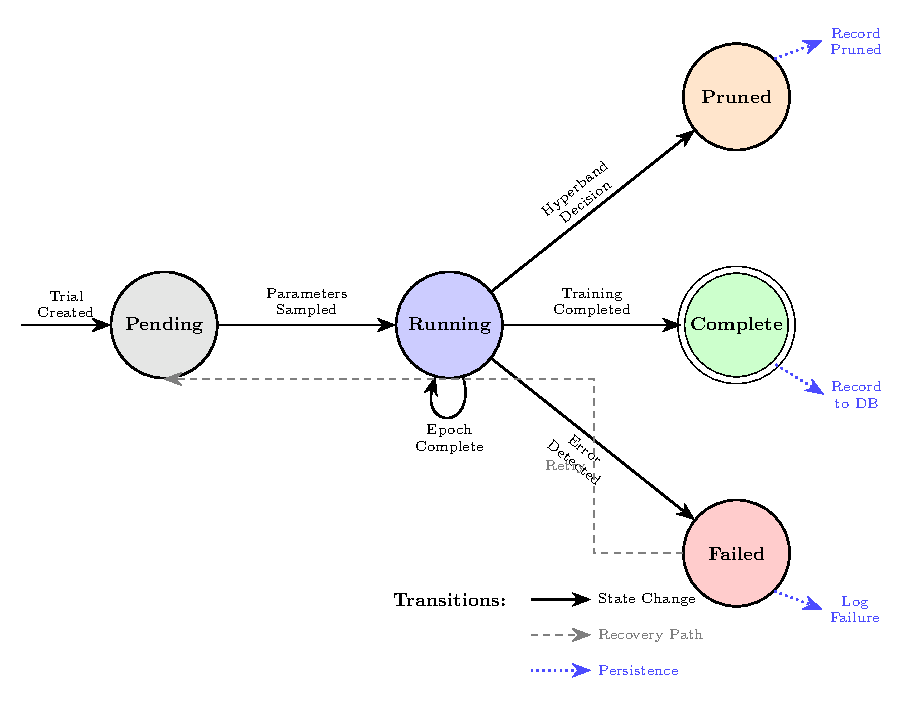
\includegraphics[width=0.85\textwidth]{figures/ch09_fig4_trial_state_machine.pdf}
\caption{Trial lifecycle state machine depicting the possible states and transitions for optimization trials. Trials begin in the Pending state upon creation, transition to Running when parameters are sampled, and terminate in one of three states: Complete (successful training and evaluation), Pruned (early termination by Hyperband), or Failed (error during execution). The self-loop on Running represents epoch completions during training. Dashed arrows indicate recovery paths for failed trials that may be retried, while dotted arrows show database persistence operations for each terminal state.}
\label{fig:trial_state_machine}
\end{figure}

\section{Reward Computation Module}
\label{sec:reward_computation}

The Reward Computation Module transforms multi-dimensional evaluation metrics into scalar reward signals suitable for consumption by the optimization algorithm, implementing the objective function that implicitly defines which parameter configurations the optimizer will prefer. The module architecture supports flexible reward formulations ranging from simple single-metric objectives through complex composite functions balancing multiple competing concerns.

\subsection{Component Calculation}

The Component Calculation subsystem computes the individual reward components that may contribute to the aggregate objective, each component capturing a distinct aspect of detector performance relevant to deployment success. Standard components include detection accuracy metrics, computational efficiency measurements, and domain adaptation indicators.

Detection accuracy components derive directly from evaluation metrics computed by the Evaluation Module, typically employing mean Average Precision at standard IoU thresholds as the primary performance indicator. Per-class Average Precision values may contribute as auxiliary components when class-specific performance requirements constrain the optimization. Precision-recall tradeoff points at fixed confidence thresholds provide alternative accuracy characterizations when detection operating points are predetermined by application requirements.

Computational efficiency components quantify the resource consumption associated with detector inference, enabling optimization that balances accuracy against deployment constraints. Inference latency measurements capture wall-clock time required for processing individual images, with the specific measurement methodology matching deployment hardware to ensure transferable efficiency estimates. Model complexity metrics including parameter counts and floating-point operation counts provide hardware-independent efficiency proxies when deployment hardware differs from evaluation infrastructure.

Domain adaptation components quantify the apparent domain shift between synthetic training data and real validation imagery, providing optimization signal that encourages generation of synthetic data whose distribution aligns with real-world conditions. Feature distribution divergence metrics compare intermediate network activations on synthetic and real images, with lower divergence indicating better domain alignment. Classifier uncertainty metrics aggregate prediction confidence statistics that may reveal distribution shift even when detection accuracy remains acceptable.

\subsection{Normalization and Smoothing}

The Normalization subsystem transforms raw reward components into standardized scales suitable for aggregation, addressing the scale incompatibilities that arise when combining metrics with different natural units and ranges. Normalization ensures that component weighting coefficients operate on comparable scales, enabling intuitive specification of relative component importance.

Range normalization maps component values to the unit interval through linear transformation based on observed or specified minimum and maximum values. Observed range normalization computes bounds from historical component distributions, automatically adapting to the realized performance range as optimization progresses. Specified range normalization employs fixed bounds derived from domain knowledge, providing stable normalization throughout optimization but requiring accurate bound specification to avoid clipped values.

Z-score normalization transforms components to zero mean and unit variance based on historical distributions, producing unbounded normalized values whose magnitudes indicate deviation from typical performance. Z-score normalization automatically adapts to performance distributions without requiring bound specification, but produces less interpretable normalized values and may exhibit instability during early optimization when historical distributions are poorly characterized.

Temporal smoothing reduces reward variance arising from stochastic training and evaluation procedures, providing more stable optimization signal at the cost of delayed response to genuine performance changes. Exponential moving average smoothing computes weighted combinations of current and historical rewards, with the smoothing coefficient balancing variance reduction against response latency. Windowed averaging computes unweighted means over recent trial sequences, providing uniform historical weighting but exhibiting step discontinuities as trials exit the averaging window.

\subsection{Degenerate Solution Detection}

The Degenerate Solution Detection subsystem identifies parameter configurations that achieve superficially strong reward values through pathological behaviors rather than genuine detection capability, flagging or penalizing such configurations to prevent optimization convergence to undesirable solutions.

Empty prediction detection identifies trials where trained detectors produce no predictions on validation imagery, a degenerate behavior that achieves perfect precision through prediction abstention. The detection mechanism examines prediction counts across validation images, flagging trials with prediction counts below configurable thresholds relative to annotation counts. Detected trials receive substantial reward penalties that ensure subsequent proposals avoid the degenerate parameter region.

Class collapse detection identifies trials where trained detectors predict only a single class regardless of actual object categories, achieving high accuracy on majority classes while failing completely on minority categories. The detection mechanism computes prediction class entropy across validation imagery, flagging trials with entropy below thresholds indicating collapsed prediction distributions. Adaptive thresholds account for natural class imbalance in validation annotations, distinguishing genuine class collapse from appropriate majority-class bias.

Confidence collapse detection identifies trials where trained detectors assign extreme confidence values to all predictions, eliminating the nuanced confidence calibration required for effective precision-recall tradeoff navigation. The detection mechanism computes confidence value variance across predictions, flagging trials with variance below thresholds indicating collapsed confidence distributions. Detected trials typically indicate training pathologies requiring hyperparameter adjustment rather than generation parameter modification.

\subsection{Logging and Monitoring}

The Logging subsystem instruments reward computation to capture comprehensive diagnostic information enabling analysis of optimization dynamics and identification of reward formulation issues. Logged information encompasses raw component values, normalized component values, aggregate rewards, and degenerate detection flags for each evaluated trial.

Component-level logging enables post-hoc analysis of which reward components drive optimization progress, informing refinement of component weights and identification of redundant or conflicting components. Temporal analysis of component trajectories reveals optimization phases where different components dominate, supporting adaptive weighting schemes that emphasize different objectives at different optimization stages.

Monitoring dashboards aggregate logging output into real-time visualizations depicting optimization progress, reward distributions, and component contributions. Standard dashboard panels include reward trajectory plots showing aggregate and component rewards over trial sequences, parameter importance rankings derived from trial comparisons, and degenerate detection alerts highlighting trials flagged for pathological behaviors.

Alert systems notify operators of optimization events requiring attention, including extended periods without reward improvement suggesting convergence or stagnation, elevated degenerate detection rates suggesting systematic parameter space issues, and infrastructure errors interrupting trial execution. Alert routing configurations specify notification channels and escalation policies appropriate to organizational requirements.

\section{Implementation Roadmap}
\label{sec:implementation_roadmap}

The implementation roadmap organizes system development into sequential phases that progressively construct operational optimization capabilities while validating assumptions and calibrating configuration parameters. The phased approach enables early detection of architectural issues, provides checkpoints for stakeholder review, and reduces risk relative to monolithic development approaches that defer integration until project completion.

\subsection{Phase 1: Infrastructure Setup}

The infrastructure setup phase establishes the foundational computational environment, software dependencies, and data management systems required by subsequent phases. Phase completion criteria include successful execution of isolated module tests and establishment of monitoring and logging infrastructure.

Computational infrastructure provisioning encompasses GPU server allocation, storage system configuration, and network connectivity establishment. GPU servers require CUDA-capable devices with sufficient memory for YOLO training at target input resolutions, with memory requirements scaling with model architecture and batch size selections. Storage systems require sufficient capacity for generated synthetic imagery, model checkpoints, and optimization databases, with typical campaigns requiring several hundred gigabytes of persistent storage.

Software dependency installation establishes Python environments with required libraries including PyTorch for neural network computation, Ultralytics for YOLO training, Optuna for optimization, and rendering backend libraries appropriate to the selected generation engine. Dependency version pinning ensures reproducible environments across development and deployment systems, with version specifications recorded in requirements manifests.

Data management infrastructure configuration establishes directory structures for synthetic imagery, validation sets, checkpoints, and logs, along with backup procedures and retention policies appropriate to operational requirements. Access control configuration restricts system access to authorized personnel while enabling automated processes to access required resources.

\subsection{Phase 2: Calibration Runs}

The calibration phase executes preliminary optimization campaigns with reduced computational budgets to validate system integration, characterize baseline performance levels, and calibrate configuration parameters. Phase completion criteria include successful end-to-end execution of optimization loops and establishment of baseline performance benchmarks.

Integration validation executes complete optimization trials to verify correct interaction among system modules, identifying interface mismatches, data format inconsistencies, and timing dependencies that impede reliable execution. Integration issues discovered during calibration are resolved before proceeding to computationally expensive main optimization campaigns.

Baseline performance characterization evaluates detector performance under default generation parameters, establishing the performance level against which optimization improvements are measured. Baseline evaluation additionally characterizes performance variance arising from stochastic training, informing confidence interval computation and convergence detection thresholds.

Configuration calibration determines appropriate values for system parameters not subject to optimization, including pruning thresholds, logging frequencies, and checkpoint intervals. Calibration experiments evaluate system behavior under candidate parameter values, selecting values that balance computational efficiency against operational reliability.

\subsection{Phase 3: Main Optimization}

The main optimization phase executes full-scale optimization campaigns with production computational budgets, discovering parameter configurations that maximize detector performance on real-world validation imagery. Phase completion criteria include convergence to stable performance levels and documentation of discovered optimal configurations.

Optimization campaign execution instantiates the Optimization Controller with production configuration and monitors execution progress through logging and dashboard infrastructure. Operator intervention addresses infrastructure issues and adjusts configuration parameters if optimization dynamics indicate suboptimal settings.

Convergence monitoring tracks performance improvement over trial sequences, identifying plateau regions indicating local optima or global convergence. Convergence detection triggers human review of optimization results, determining whether discovered configurations achieve acceptable performance or whether additional optimization effort is warranted.

Result documentation records optimal parameter configurations, achieved performance levels, and optimization trajectories for subsequent analysis and reporting. Documentation includes sufficient detail to enable reproduction of optimization campaigns and interpretation of results by stakeholders unfamiliar with system internals.

\subsection{Phase 4: Final Validation}

The final validation phase subjects discovered optimal configurations to rigorous evaluation establishing confidence in deployment readiness. Phase completion criteria include statistical validation of performance claims and documentation suitable for deployment approval processes.

Extended evaluation expands assessment beyond the validation set employed during optimization, evaluating detector performance on held-out test imagery and optionally on imagery from related domains. Extended evaluation guards against overfitting to validation set idiosyncrasies and characterizes generalization capabilities relevant to deployment success.

Statistical validation applies hypothesis testing procedures to compare optimal configurations against baseline configurations and alternative optimization approaches, establishing statistically significant performance improvements. Validation reports document achieved confidence levels and characterize remaining uncertainty in performance estimates.

Deployment documentation produces comprehensive records of optimal configurations, performance characteristics, and operational requirements suitable for handoff to deployment teams. Documentation includes configuration files, trained model weights, and operational procedures enabling deployment teams to instantiate operational detectors without requiring optimization expertise.

\begin{table}[htbp]
\centering
\caption{Implementation Roadmap Timeline and Milestones}
\label{tab:implementation_timeline}
\begin{tabular}{p{2cm}p{3.5cm}p{3cm}p{5cm}}
\toprule
\textbf{Phase} & \textbf{Duration} & \textbf{Compute Budget} & \textbf{Key Deliverables} \\
\midrule
Phase 1 & 1--2 weeks & Minimal & Configured infrastructure, module tests passing, monitoring operational \\
\addlinespace
Phase 2 & 1--2 weeks & 10--20 trials & Integration validated, baseline performance characterized, parameters calibrated \\
\addlinespace
Phase 3 & 2--4 weeks & 50--100 trials & Converged optimization, optimal configurations documented, performance targets achieved \\
\addlinespace
Phase 4 & 1--2 weeks & 5--10 trials & Statistical validation complete, deployment documentation delivered, approval obtained \\
\bottomrule
\end{tabular}
\end{table}

\begin{figure}[htbp]
\centering
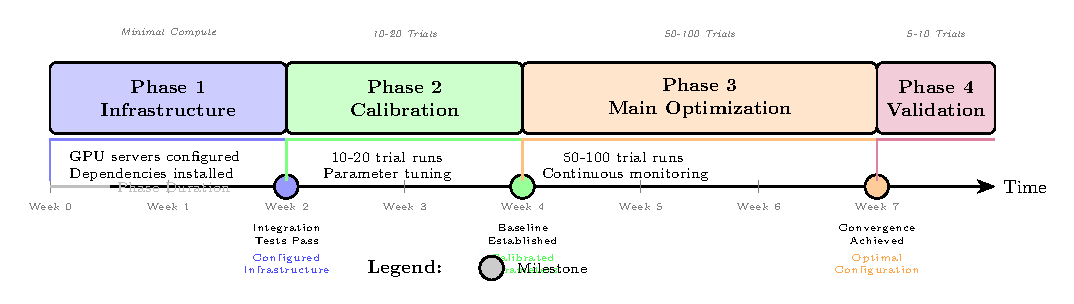
\includegraphics[width=\textwidth]{figures/ch09_fig3_implementation_roadmap.pdf}
\caption{Implementation roadmap timeline visualization showing the four phases of system deployment. Each phase is represented with its duration, computational budget, and key milestones. Phase 1 (Infrastructure) establishes the computational environment with minimal compute requirements. Phase 2 (Calibration) runs initial trials to establish baselines. Phase 3 (Main Optimization) executes the primary optimization campaign with 50--100 trials. Phase 4 (Validation) performs statistical validation and prepares deployment documentation. Milestones mark the completion of each phase with specific deliverables.}
\label{fig:implementation_roadmap}
\end{figure}

\section{Practical Considerations}
\label{sec:practical_considerations}

Production deployment of optimization systems encounters practical challenges extending beyond algorithmic correctness, requiring engineering solutions that ensure reliable operation under real-world conditions. This section addresses common operational challenges and presents strategies for robust system operation.

\subsection{Checkpointing and Recovery}

Robust checkpointing strategies ensure that system failures result in bounded work loss rather than complete campaign restart. The checkpointing architecture captures complete system state at configurable intervals, enabling recovery to any checkpointed state with guaranteed consistency.

Study-level checkpointing persists Optuna study state to durable storage, capturing completed trial results, pending trial states, and sampler internal state. Database storage backends provide automatic checkpointing through transaction logging, while file-based storage requires explicit checkpoint operations. Recovery from study checkpoints restores complete optimization history, enabling continued optimization from the last persisted state.

Model-level checkpointing persists YOLO training state at epoch boundaries, capturing model weights, optimizer state, and training progress. Checkpoint frequency balances recovery granularity against storage and I/O overhead, with per-epoch checkpointing appropriate for production campaigns where recovery time exceeds epoch duration. Recovery from model checkpoints resumes training from the checkpointed epoch, avoiding repetition of completed training work.

Data-level checkpointing records generated synthetic imagery and annotations to persistent storage, enabling training resumption without regeneration. Corpus generation typically dominates checkpoint storage requirements, motivating retention policies that balance storage consumption against regeneration cost. Checksums enable verification of corpus integrity after recovery, detecting corruption that would contaminate subsequent training.

\subsection{Handling Failed Training Runs}

Training failures arising from numerical instabilities, resource exhaustion, or software errors require graceful handling that preserves optimization progress while avoiding systematic bias from failure patterns. The failure handling strategy distinguishes recoverable failures warranting retry from persistent failures requiring parameter adjustment.

Automatic retry policies specify the maximum number of retry attempts before declaring trial failure, along with backoff intervals between attempts that may permit transient resource contention to resolve. Retry attempts optionally modify training configuration through batch size reduction, learning rate adjustment, or random seed changes that may circumvent failure-inducing conditions.

Failure penalty assignment determines the objective value recorded for persistently failed trials, influencing subsequent sampling behavior. Pessimistic penalties assign values worse than any observed successful trial, strongly discouraging sampling in failure-inducing parameter regions. Neutral penalties exclude failed trials from sampler modeling, preventing failure patterns from biasing proposals while forgoing the information that failures provide about parameter space structure.

Failure pattern analysis examines failure rates across parameter regions, identifying systematic failure modes that warrant parameter space constraints or configuration adjustments. Persistent failures concentrated in specific parameter subspaces may indicate incompatible generation parameters, overly aggressive training configurations, or infrastructure limitations requiring architectural revision.

\subsection{Warm-Starting from Prior Knowledge}

Warm-starting strategies accelerate optimization convergence by initializing from prior knowledge accumulated through previous campaigns, domain expertise, or related optimization problems. Effective warm-starting can reduce iteration counts by thirty to fifty percent compared to cold-starting, substantially reducing computational expenditure.

Historical trial injection populates new studies with results from previous optimization campaigns, providing the sampler with prior observations that inform initial proposals. Injected trials must be compatible with current parameter space definitions, potentially requiring transformation when parameter spaces differ between campaigns. Compatibility verification prevents injection of incompatible trials that would corrupt sampler modeling.

Expert configuration seeding initializes optimization with parameter configurations derived from domain expertise or published best practices, ensuring that known-good configurations receive evaluation regardless of sampler proposals. Seeded configurations are enqueued as pending trials that execute before sampler-generated proposals, providing immediate evaluation of expert knowledge.

Transfer learning from related problems leverages optimization results from similar but distinct domains, potentially informing proposals even when target domain differs from source domain. Transfer effectiveness depends on domain similarity, with conservative transfer strategies that downweight source observations appropriate when domain relationships are uncertain.

\subsection{Logging and Visualization}

Comprehensive logging enables retrospective analysis of optimization behavior, supporting both immediate debugging and long-term system improvement. The logging architecture captures structured records at multiple granularities from individual function invocations through complete optimization campaigns.

Structured logging employs standardized formats that enable automated parsing and aggregation, with JSON formatting providing flexibility for heterogeneous log entries. Log records include timestamps, log levels, component identifiers, and structured payloads capturing event-specific information. Centralized log aggregation enables correlation analysis across distributed system components.

Real-time visualization presents optimization progress through continuously-updated dashboards displaying key metrics and system status. Standard dashboard elements include objective value trajectories, parameter distributions, trial status summaries, and resource utilization indicators. Interactive visualization enables drill-down from aggregate views to individual trial details.

Post-hoc analysis tools process logged data to extract insights informing system improvement, including parameter importance analysis identifying high-impact parameters, convergence analysis characterizing optimization efficiency, and failure analysis identifying systematic issues requiring architectural attention.

\subsection{Debugging Strategies}

Systematic debugging strategies accelerate issue resolution when optimization behavior deviates from expectations, whether through failure to improve, convergence to suboptimal configurations, or erratic optimization dynamics. Effective debugging leverages comprehensive logging to localize issues and reproduce failures in controlled conditions.

Reproducibility enforcement ensures that debugging investigations can recreate observed behaviors, requiring complete capture of random seeds, software versions, and environmental conditions. Reproducibility verification confirms that recorded conditions suffice to recreate behavior before commencing investigation.

Isolation strategies narrow issue scope by disabling or mocking system components to determine which module contributes to observed misbehavior. Progressive isolation begins with coarse component boundaries and proceeds to finer granularities as investigation narrows the likely issue location.

Reference implementations provide known-correct behavior against which production system output can be compared, identifying discrepancies that localize issues. Reference implementations sacrifice efficiency for clarity and correctness, enabling verification without requiring comprehension of production optimization.

\section{Recommended Tools and Libraries}
\label{sec:recommended_tools}

Tool selection significantly impacts implementation effort, operational reliability, and extensibility to future requirements. This section presents recommendations based on evaluation of available options against the specific requirements of synthetic data optimization for object detection.

\subsection{Optuna for Optimization}

Optuna provides the optimization algorithm implementation recommended for synthetic data parameter tuning, offering mature implementations of Tree-structured Parzen Estimation, Hyperband pruning, and distributed optimization coordination with minimal integration effort.

The TPE sampler implementation handles mixed parameter types including continuous, discrete, and categorical parameters with appropriate kernel density estimation for each type. Multivariate modeling captures parameter correlations that improve sample efficiency when parameters interact. Automatic handling of conditional parameters enables complex parameter space definitions with dependencies among parameters.

The pruning framework provides Hyperband and successive halving implementations that integrate seamlessly with training callbacks, enabling early termination decisions based on intermediate training metrics. Pruning configuration requires minimal hyperparameter specification, with sensible defaults appropriate for most optimization problems.

The distributed optimization capabilities enable parallel trial execution across multiple workers sharing study state through database storage backends. Worker coordination ensures consistent study state despite concurrent access, with transaction isolation preventing conflicts between simultaneous parameter proposals.

\subsection{Ultralytics for YOLO}

The Ultralytics library provides YOLO implementation recommended for detector training, offering production-grade implementations of contemporary YOLO architectures with consistent training and inference APIs.

Architecture support encompasses YOLOv5, YOLOv8, and subsequent architecture revisions, enabling architecture selection based on accuracy-efficiency tradeoffs appropriate to deployment requirements. Pretrained weights for standard architectures enable transfer learning that accelerates training convergence and improves final accuracy.

Training utilities implement contemporary training techniques including mosaic augmentation, automatic learning rate finding, and mixed-precision training that maximize accuracy within computational constraints. Export utilities produce optimized model formats for deployment including ONNX, TensorRT, and CoreML.

The callback system enables integration with external monitoring and control systems, providing hooks for training progress reporting, intermediate validation, and early termination. Callback-based integration preserves library upgrade compatibility by avoiding modifications to library internals.

\subsection{Blender and Isaac Sim for Generation}

Blender and NVIDIA Isaac Sim provide complementary synthetic data generation capabilities addressing different requirements along the flexibility-capability tradeoff.

Blender's open-source license eliminates licensing costs while providing comprehensive three-dimensional modeling, animation, and rendering capabilities through an extensive Python API. The Cycles renderer provides physically-based path tracing producing photorealistic output, while the Eevee renderer provides faster rasterization-based rendering suitable for rapid iteration. Community extensions provide domain-specific functionality for common synthetic data generation requirements.

Isaac Sim provides production-grade synthetic data generation integrated with NVIDIA's Omniverse platform, offering advanced physics simulation, photorealistic rendering through RTX acceleration, and extensive asset libraries with simulation-ready models. The Replicator API provides high-level abstractions for common generation tasks including randomization, annotation, and format conversion. Enterprise support provides assistance for production deployment requirements.

The backend abstraction layer enables use of either generation engine through consistent interfaces, with backend selection based on available hardware, licensing constraints, and domain-specific requirements. Hybrid approaches employing different backends for different generation tasks combine the strengths of each platform.

\subsection{Ray for Parallelization}

Ray provides distributed computing capabilities that enable parallel execution of optimization trials, generation processes, and training workloads across heterogeneous computational resources.

The task-based programming model enables straightforward parallelization of independent operations without explicit coordination logic, with the Ray runtime handling task scheduling, data movement, and failure recovery. Task dependencies expressed through object references enable automatic pipeline execution when dependent tasks produce required inputs.

The actor-based programming model enables stateful computations that maintain context across method invocations, appropriate for generation engines and training processes that benefit from persistent state. Actor lifecycle management handles initialization, checkpointing, and recovery automatically.

Integration with Optuna enables distributed optimization with Ray-based parallel trial execution, scaling optimization throughput linearly with available computational resources while maintaining optimization algorithm correctness through centralized study state management.

\begin{table}[htbp]
\centering
\caption{Comparison of Recommended Tools and Alternatives}
\label{tab:tool_comparison}
\begin{tabular}{p{2.5cm}p{3.5cm}p{3.5cm}p{4cm}}
\toprule
\textbf{Category} & \textbf{Recommended} & \textbf{Alternatives} & \textbf{Selection Rationale} \\
\midrule
Optimization & Optuna & Hyperopt, BoTorch, SMAC & Mature TPE/Hyperband, excellent distributed support, active development \\
\addlinespace
Detection & Ultralytics & Detectron2, MMDetection & Production-ready YOLO, consistent API, comprehensive documentation \\
\addlinespace
Generation & Blender + Isaac Sim & Unity Perception, Unreal Engine & Flexibility + capability coverage, strong Python integration \\
\addlinespace
Parallelization & Ray & Dask, multiprocessing & Unified task/actor model, Optuna integration, enterprise support \\
\addlinespace
Logging & TensorBoard + W\&B & MLflow, Neptune & Wide adoption, real-time visualization, experiment comparison \\
\addlinespace
Storage & PostgreSQL & SQLite, MySQL & Concurrent access, transaction support, mature tooling \\
\bottomrule
\end{tabular}
\end{table}

\section{Main Optimization Loop Algorithm}
\label{sec:main_algorithm}

The main optimization loop algorithm integrates the modules described in preceding sections into a complete procedure for discovering optimal synthetic data generation parameters. The algorithm implements the BOHB optimization strategy with multi-fidelity evaluation through Hyperband pruning.

\begin{algorithm}[htbp]
\caption{Main Synthetic Data Optimization Loop}
\label{alg:main_optimization}
\begin{algorithmic}[1]
\Require Parameter space $\Theta$, validation set $\mathcal{V}$, computational budget $B$
\Ensure Optimal parameters $\boldsymbol{\theta}^*$, best objective value $r^*$
\State Initialize study $\mathcal{S}$ with TPE sampler and Hyperband pruner
\State Load prior trials from persistent storage if available
\State $r^* \gets -\infty$, $\boldsymbol{\theta}^* \gets \text{None}$
\While{budget remaining and not converged}
    \State $\boldsymbol{\theta} \gets \text{TPESampler.propose}(\mathcal{S})$ \Comment{Propose parameter configuration}
    \State $\mathcal{D}_{\text{synth}} \gets \text{GenerateSyntheticData}(\boldsymbol{\theta})$ \Comment{Generate training corpus}
    \If{$\text{QualityCheck}(\mathcal{D}_{\text{synth}})$ fails}
        \State Record failed trial, \textbf{continue}
    \EndIf
    \State Initialize YOLO model $\mathcal{M}$
    \For{epoch $e = 1$ to $E_{\text{max}}$}
        \State Train $\mathcal{M}$ for one epoch on $\mathcal{D}_{\text{synth}}$
        \State $m_e \gets \text{IntermediateValidation}(\mathcal{M})$
        \State Report $m_e$ to pruner
        \If{$\text{HyperbandPruner.should\_prune}(m_e, e)$}
            \State Record pruned trial, \textbf{break}
        \EndIf
    \EndFor
    \If{trial not pruned}
        \State $\mathcal{M}_{\text{final}} \gets \text{LoadBestCheckpoint}()$
        \State metrics $\gets \text{EvaluateOnValidation}(\mathcal{M}_{\text{final}}, \mathcal{V})$
        \State $r \gets \text{ComputeReward}(\text{metrics})$
        \State Record completed trial with objective $r$
        \If{$r > r^*$}
            \State $r^* \gets r$, $\boldsymbol{\theta}^* \gets \boldsymbol{\theta}$
        \EndIf
    \EndIf
    \State Persist study state to database
    \State Update convergence statistics
\EndWhile
\State \Return $\boldsymbol{\theta}^*$, $r^*$
\end{algorithmic}
\end{algorithm}

The algorithm begins by initializing an Optuna study configured with the TPE sampler for parameter proposal and the Hyperband pruner for early termination. Prior trial results are loaded from persistent storage if available, enabling warm-starting from previous optimization campaigns or recovery from interrupted executions.

The main loop iterates until the computational budget is exhausted or convergence criteria are satisfied. Each iteration proposes a parameter configuration through the TPE sampler, generates a synthetic training corpus according to the proposed parameters, validates corpus quality through automated checks, trains a YOLO detector on the generated corpus with periodic pruning evaluations, evaluates the trained detector on real validation imagery, computes a scalar reward from evaluation metrics, and records the complete trial to persistent storage.

Early termination through Hyperband pruning substantially reduces computational expenditure by abandoning unpromising trials before training completion. The pruner evaluates intermediate validation metrics at configurable epoch intervals, comparing trial performance against the distribution of previously observed intermediate metrics to determine whether continuation is warranted. Pruned trials contribute to the sampler's performance model, informing subsequent proposals to avoid parameter regions associated with pruned trials.

\section{Data Flow Diagram}
\label{sec:data_flow_diagram}

The following diagram depicts the flow of data through the optimization system, illustrating the transformations applied at each stage and the feedback loop that enables iterative parameter refinement.

\begin{figure}[htbp]
\centering
\begin{tikzpicture}[
    node distance=1.5cm and 2cm,
    data/.style={rectangle, draw=black, thick, fill=yellow!20, minimum width=2.5cm, minimum height=0.8cm, align=center, rounded corners=2pt},
    process/.style={rectangle, draw=black, thick, fill=blue!15, minimum width=3cm, minimum height=1cm, align=center},
    decision/.style={diamond, draw=black, thick, fill=green!15, minimum width=2cm, minimum height=1cm, align=center, aspect=2},
    arrow/.style={->, thick, >=stealth}
]

% Left column - Data
\node[data] (params) {Parameter Vector\\$\boldsymbol{\theta}$};
\node[data, below=of params] (config) {Generation\\Config};
\node[data, below=of config] (images) {Synthetic\\Images};
\node[data, below=of images] (annot) {YOLO\\Annotations};
\node[data, below=of annot] (corpus) {Training\\Corpus};

% Middle column - Processes
\node[process, right=2.5cm of params] (sampler) {TPE Sampler};
\node[process, right=2.5cm of config] (generator) {Blender/Isaac\\Renderer};
\node[process, right=2.5cm of images] (annotator) {Annotation\\Generator};
\node[process, right=2.5cm of corpus] (trainer) {YOLO\\Trainer};

% Right column - More data and processes
\node[data, right=2.5cm of sampler] (history) {Trial\\History};
\node[data, right=2.5cm of trainer] (model) {Trained\\Model};
\node[process, below=of model] (evaluator) {Evaluation\\Module};
\node[data, below=of evaluator] (metrics) {Performance\\Metrics};
\node[process, below=of metrics] (reward) {Reward\\Computation};
\node[data, below=of reward] (signal) {Reward\\Signal $r$};

% Arrows
\draw[arrow] (sampler) -- (params);
\draw[arrow] (params) -- (config);
\draw[arrow] (config) -- (generator);
\draw[arrow] (generator) -- (images);
\draw[arrow] (images) -- (annotator);
\draw[arrow] (annotator) -- (annot);
\draw[arrow] (annot) -- (corpus);
\draw[arrow] (corpus) -- (trainer);
\draw[arrow] (trainer) -- (model);
\draw[arrow] (model) -- (evaluator);
\draw[arrow] (evaluator) -- (metrics);
\draw[arrow] (metrics) -- (reward);
\draw[arrow] (reward) -- (signal);

% Feedback loop
\draw[arrow] (signal.west) -- ++(-1,0) |- ([yshift=0.5cm]sampler.west) -- (sampler.west);
\draw[arrow] (history) -- (sampler);

% Validation set input
\node[data, left=1.5cm of evaluator] (valset) {Real\\Validation Set};
\draw[arrow] (valset) -- (evaluator);

\end{tikzpicture}
\caption{Data flow diagram illustrating transformations from parameter proposals through synthetic data generation, model training, evaluation, and reward computation. The feedback loop from reward signal to TPE sampler enables iterative refinement of parameter proposals based on accumulated trial history.}
\label{fig:data_flow}
\end{figure}

\section{Chapter Summary}

This chapter has presented a comprehensive treatment of the system architecture and implementation considerations for reinforcement learning-optimized synthetic data generation targeting YOLO object detection training. The architectural design organizes functionality into six principal modules whose interactions implement the closed-loop optimization paradigm central to the methodology developed throughout this text.

The Synthetic Data Generation Module translates abstract parameter specifications into concrete training imagery through integration with Blender and Isaac Sim rendering backends, implementing the domain randomization strategies essential for producing synthetic corpora that induce detectors capable of real-world generalization. The YOLO Training Module encapsulates neural network training workflows through Ultralytics integration, providing consistent interfaces regardless of specific architecture variant while exposing callback interfaces that enable pruning decisions based on intermediate training dynamics.

The Evaluation Module addresses the statistical challenges inherent in performance assessment with limited real-world validation imagery, implementing bootstrap confidence computation and class-balanced metrics that provide reliable optimization signals despite validation set sizes as small as fifty images. The Reward Computation Module transforms multi-dimensional evaluation results into scalar optimization objectives, implementing normalization, smoothing, and degenerate solution detection that ensure robust optimization dynamics.

The Optimization Controller implements the BOHB algorithm through Optuna integration, combining Tree-structured Parzen Estimation for informed parameter proposal with Hyperband pruning for early termination of unpromising trials. Database persistence enables recovery from interruptions, distributed optimization across multiple workers, and warm-starting from prior accumulated knowledge.

The implementation roadmap organizes development into phases that progressively construct operational capabilities while validating assumptions and calibrating configuration parameters. Practical considerations including checkpointing strategies, failure handling policies, and debugging approaches address the engineering challenges that distinguish production deployments from research prototypes.

The recommended tool stack comprising Optuna, Ultralytics, Blender, Isaac Sim, and Ray provides production-grade implementations of all required functionality, enabling practitioners to focus implementation effort on domain-specific adaptations rather than foundational infrastructure. The algorithmic specification and architectural diagrams presented in this chapter provide complete blueprints for constructing operational optimization systems that realize the theoretical developments presented throughout preceding chapters.
